\documentclass{article}
\usepackage{tikz}
\usetikzlibrary{positioning}
\usepackage{amsmath,amssymb}
%Title
\title{Bipartito o Ciclo}
\author{Daniel Bustos}
\begin{document}
\maketitle

Sea $G = (V,E)$ con $|V| = n$. Queremos probar que: $\forall v \in V$, $G-v$ es bipartito $\leftrightarrow$ $G$ es bipartito o ciclo impar.

Probemos la ida:

\textbf{$\forall v \in V$, $G-v$ es bipartito $\rightarrow$ $G$ es bipartito o ciclo impar.}\\ 

Probémoslo por el contrarrecíproco.\\
\textbf{$G$  no es bipartito ni es ciclo impar $\rightarrow \exists v \in V: G-v $ no es bipartito}\\\\

Supongamos que $G$ no es bipartito ni ciclo impar. Esto nos deja dos casos:
\begin{itemize}


\item Si es ciclo par, podemos tomar los vértices impares, y los impares por separado. Dentro de cada uno de estos no hay relaciones, por lo tanto, $G$ es bipartito, lo cual es absurdo porque dijimos que $G$ no lo era. Luego, este caso no puede ocurrir. Por ejemplo:

\begin{center}
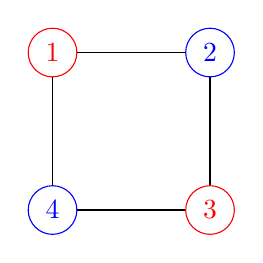
\begin{tikzpicture}
  \node[circle,draw,red] (1) at (0,0) {1};
  \node[circle,draw,blue] (2) at (2,0) {2};
  \node[circle,draw,red] (3) at (2,-2) {3};
  \node[circle,draw,blue] (4) at (0,-2) {4};
  
  \draw (1) -- (2);
  \draw (2) -- (3);
  \draw (3) -- (4);
  \draw (4) -- (1);
\end{tikzpicture}
\end{center}

Se observa que podemos tomar las biparticiones $\{1,3\}$ y $\{2,4\}$ respectivamente.

\item $G$ no es ciclo: En este caso debemos usar algo un poco mas potente. Usaremos el siguiente teorema : \\ 
\textbf{ Un grafo G no es bipartito  $\leftrightarrow \exists$ un ciclo impar en G}\\
 A partir de esto podemos tomar otros dos subscuentes casos \\\\
\newpage
\item Ciclo impar con cosas sueltas afuera:
\begin{center}
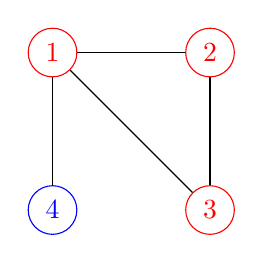
\begin{tikzpicture}
  \node[circle,draw,red] (1) at (0,0) {1};
  \node[circle,draw,red] (2) at (2,0) {2};
  \node[circle,draw,red] (3) at (2,-2) {3};
  \node[circle,draw,blue] (4) at (0,-2) {4};
  
  \draw (1) -- (2);
  \draw (2) -- (3);
  \draw (3) -- (1);
  \draw (4) -- (1);
\end{tikzpicture}
\end{center}
En este caso podemos tomar remover algun vértices de afuera y como claramente nos sigue quedando un ciclo impar, entonces es bipartito por el teorema anterior.
		
\item Ciclo impar sin nada afuera, pero aristas internas extras
\begin{center}

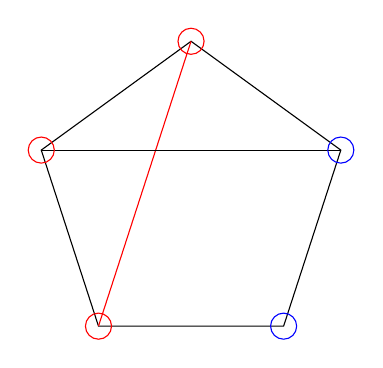
\begin{tikzpicture}
% Define the vertices of the pentagon
\coordinate (P1) at (90:2);
\coordinate (P2) at (162:2);
\coordinate (P3) at (234:2);
\coordinate (P4) at (306:2);
\coordinate (P5) at (18:2);

% Draw the edges of the pentagon
\draw (P1) -- (P2) -- (P3) -- (P4) -- (P5) -- cycle;

% Draw internal edges
\draw[red] (P1) -- (P3);
\draw (P2) -- (P5);

% Draw the vertices
\foreach \i in {1,...,5}{
	\ifnum \i<4    
    	  \node[circle,draw,red] at (P\i) {};
    \else
      \node[circle,draw,blue] at (P\i) {};
     \fi
}
\end{tikzpicture}
\end{center}
Tomemos una arista interna de este grafo. Observemos que a partir de esta  podemos definir al menos dos ciclos con las demas vertices de G. Uno del "lado izquierdo" de la arista y otro del "derecho". Veamos que alguno de estos dos ciclos debe ser impar, contando cuantos nodos pueden tener estos dos ciclos:

Sabemos que nuestro grafo tiene $2k + 1$(cantidad impar) de nodos, para algún $k \in \mathbb{N}_0$. Después de elegir la arista que nos da nuestras dos particiones, llamemos $C1$ y $C2$ a los ciclos que se nos forman.

La cantidad de vértices, tanto en $C1$ y $C2$, son los vértices de la arista que elegimos más los demas vertices del grafo, que esten en cada lado respectivamente. Llamemos $v$ y $w$ a estos dos vértices, luego la cantidad de vértices en $C1$ y $C2$ es:
\[|V(C1)| = 2 + |C1 - \{v,w\}|, \quad |V(C2)| = 2 + |C2 - \{v,w\}|\]

Por ende debe cumplirse que la cantidad de vértices en nuestro grafo $G$ es:  $ |V(G)| = |V(C2)| + |V(C1)| - 2$.\\
\textbf{OBS:}\textit{ debemos restarle 2 , ya que de otra manera estariamos contando los vertices que nos generan nuestra particion de manera repetida}

Como sabemos que $|V(G)|$ es un número impar, necesariamente \textbf{uno y solo uno de nuestros dos ciclos debe tener cantidad impar de vértices}. De otro modo $G$ tendría cantidad par de vértices, y dijimos que $G$ es un ciclo impar con aristas adicionales. Por lo tanto, en este caso de grafo, podemos siempre tomar un vértice de nuestra "partición par" de ciclos, y nos sigue quedando un ciclo impar en $G$, que por el teorema, nos dice que es bipartito.\\

Habiendo visto que en todos los casos se cumple, queda demostrada la ida

\end{itemize}
Probemos la vuelta: \\

\textbf{$G$ es bipartito o ciclo impar. $\rightarrow \forall v \in V$, $G-v$ es bipartito} 
\begin{itemize}
\item \textbf{Si G es ciclo impar} sus aristas son de la forma:

\[\forall 0 < i < n,\ v_i \in V(g) : (v_i,v_{i+1}) \in E(G) \land   (v_n,v_0) \in E(G) \]

Luego , podemos tomar cualquier vertice y removerlo. Generandonos las biparticiones de los $v_i$  pares,  y $v_i'$ y impares, que por ser ciclo G original ciclo impar, necesariamente no estan conectados entre si. Como podemos remover cualquier vertice y esto vale, se cumple lo que queriamos ver.

\begin{figure}[h]
\centering
\begin{minipage}{0.4\textwidth}
\centering
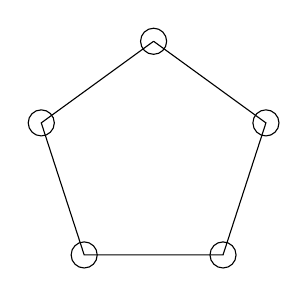
\begin{tikzpicture}
% Define the vertices of the odd cycle
\coordinate (P1) at (90:1.5);
\coordinate (P2) at (162:1.5);
\coordinate (P3) at (234:1.5);
\coordinate (P4) at (306:1.5);
\coordinate (P5) at (18:1.5);

% Draw the edges of the odd cycle
\draw (P1) -- (P2) -- (P3) -- (P4) -- (P5) -- (P1);

% Draw the vertices
\foreach \i in {1,...,5}
    \node[circle,draw] at (P\i) {};
\end{tikzpicture}
\caption*{Grafo original: Ciclo Impar}
\end{minipage}
\hspace{1cm}
\begin{minipage}{0.4\textwidth}
\centering
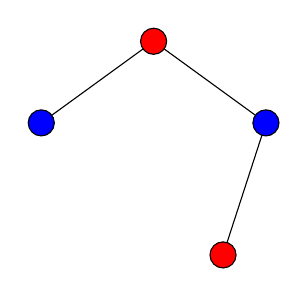
\begin{tikzpicture}[vertex/.style={draw,circle,fill=black,minimum size=3pt,inner sep=0pt}]
% Define the vertices of the modified graph
\coordinate (P1) at (90:1.5);
\coordinate (P2) at (162:1.5);
\coordinate (P3) at (306:1.5);
\coordinate (P5) at (18:1.5);

% Draw the edges of the modified graph
\draw (P1) -- (P2);
\draw (P3) -- (P5);
\draw (P5) -- (P1);

% Draw the vertices
\foreach \i/\color in {1/red,2/blue,3/red,5/blue}
    \node[circle,draw, fill=\color] at (P\i) {};
\end{tikzpicture}
\caption*{Grafo con vertice removido}
\end{minipage}
\end{figure}
\begin{center}
Veamos ahora el otro caso
\end{center}
\newpage
\item \textbf{Si G es bipartito} tenemos nuestras dos biparticiones V1 y V2. Como ningun elemento de V1 o V2 esta relacionado con elementos de su mismo grupo, podemos perfectamente remover cualquier vertice del grafo, y las biparticiones siguen valiendo, ya que removiendo vertices es claro que no apareceran ningunas conexiones nuevas entre ninguno dos vertices, en particular entre ninguno de las biparticiones $\square$.

\begin{figure}[!ht]
    \centering
    \begin{minipage}[b]{0.45\textwidth}
        \centering
        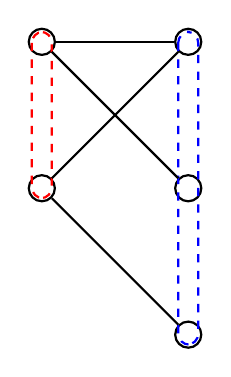
\begin{tikzpicture}[node distance=1.5cm, thick]
        % Nodes in the first part
        \node[circle, draw] (A1) {};
        \node[circle, draw, below=of A1] (A2) {};
        % Nodes in the second part
        \node[circle, draw, right=of A1] (B1) {};
        \node[circle, draw, below=of B1] (B2) {};
        \node[circle, draw, below=of B2] (B3) {};
        % Encircle the two parts
        \draw[dashed, rounded corners, red] (A1.north west) rectangle (A2.south east);
        \draw[dashed, rounded corners, blue] (B1.north west) rectangle (B3.south east);
        % Edges
        \draw (A1) -- (B1);
        \draw (A1) -- (B2);
        \draw (A2) -- (B1);
        \draw (A2) -- (B3);
        \end{tikzpicture}
        \caption{Grafo con nodo menos}
        \label{fig:graph1}
    \end{minipage}
    \hfill
    \begin{minipage}[b]{0.45\textwidth}
        \centering
        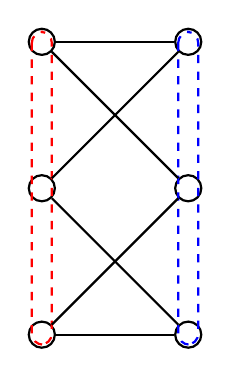
\begin{tikzpicture}[node distance=1.5cm, thick]
        % Nodes in the first part
        \node[circle, draw] (A1) {};
        \node[circle, draw, below=of A1] (A2) {};
        \node[circle, draw, below=of A2] (A3) {};
        % Nodes in the second part
        \node[circle, draw, right=of A1] (B1) {};
        \node[circle, draw, below=of B1] (B2) {};
        \node[circle, draw, below=of B2] (B3) {};
        % Encircle the two parts
        \draw[dashed, rounded corners, red] (A1.north west) rectangle (A3.south east);
        \draw[dashed, rounded corners, blue] (B1.north west) rectangle (B3.south east);
        % Edges
        \draw (A1) -- (B1);
        \draw (A1) -- (B2);
        \draw (A2) -- (B1);
        \draw (A2) -- (B3);
        \draw (A3) -- (B2);
        \draw (A3) -- (B3);
        \end{tikzpicture}
        \caption{Grafo Bipartito}
        \label{fig:graph2}
    \end{minipage}
\end{figure}



\end{itemize}



\end{document}
